%%%%%%%%%%%%%%%%%%%%%%%%%%%%%%%%%%%%%%%%%
% Beamer Presentation
% LaTeX Template
% Version 2.0 (10/06/16)
%
% Attention:
% 0. The self-defined font is used, because 'Calibri' is 
% not supported in the latex font packages. 'LuaLatex'
% should be used.
% 1. This template has been generated according to 
% the Power Point template of LUMC in 2016. 
% 2. This is generated purely with images as the 
% background.
% 3. The bullet point color was used purely for personal 
% preference. 
% 4. Any more adding to the template are welcome. 
% 5.In order to use the navigation bar, the title 
% for each section should not be to long. 
% 6.Adding animation is possible. I prefer to add another
% pdf file with:
% \animategraphics[parameters]{1}{fname}{startnum}{endnum}
% 7. This is my first template, the files might be not  
% well organized, sorry for that. 
% 
% Author:
% Shengnan Liu
% sliu729@gmail.com
% Division Medical imaging processing, 
% Leiden University Medical Center
% 
%%%%%%%%%%%%%%%%%%%%%%%%%%%%%%%%%%%%%%%%%
% Modification Log:
% Generated by Shengnan Liu on 21-01-2016
% Cleaned up for further usage on 10-06-2016
%%%%%%%%%%%%%%%%%%%%%%%%%%%%%%%%%%%%%%%%%
\documentclass[aspectratio=169]{beamer}
\beamertemplatenavigationsymbolsempty%
\usepackage{textpos}
\usefonttheme[onlymath]{serif}
\usepackage{eso-pic}
\usepackage{fontspec}
\usepackage{multirow}
\usepackage{booktabs}
\usepackage{textcomp}
\usepackage{listings}
\setsansfont{Linux Biolinum O}
%\setmainfont{Gentium}
\usetheme{Rochester}% theme
\usecolortheme{seahorse}
\colorlet{beamer@blendedblue}{green!40!black}
%\setbeamertemplate{navigation symbols}{}
%\setbeamertemplate{footline}[frame number]
\setbeamertemplate{footline}{% hide total number of slides
  \hfill% 
  \usebeamercolor[fg]{page number in head/foot}% 
  \usebeamerfont{page number in head/foot}% 
  \insertframenumber%
  \kern1em\vskip2pt% 
}
\setbeamertemplate{itemize items}[circle]
\hypersetup{
    colorlinks = true,
    urlcolor = cyan
}

%\addtobeamertemplate{frametitle}{}{%
%\begin{textblock*}{100mm}(.80\textwidth,-1.55cm)
%
\includegraphics[height=1.5cm]{figures/csu-logo.png}
%\end{textblock*}}

\title{Large Matrix Manipulation for Unfolding Optimization}
\date[today]{\today}
\author{Shih-Kai Lin}
\institute{Colorado State University}
\usepackage{multicol} % 
%\usepackage{animate}  % animation
\usepackage{amsmath,amsfonts,amssymb} % This makes the equations appears better 
\begin{document}
%The title
\begin{frame}
\titlepage
\end{frame}


% Adding note that cannot be seen
\note[itemize]{
\item Good morning everyone. Today I would like to present the work that were submitted to SPIE proceeding photonics west. 
\item point 2
}

\begin{frame}{Overview}
  \begin{itemize}
    \item I have been dealing with covariance matrices of size $6776\times 6776$ for optimizing the number of iterations in iterative unfolding.
    \item In this study, RooUnfold is used to calculate the covariance matrix.
    \item Matrix manipulation is done with \texttt{PyROOT}, \texttt{root\_numpy}, and \texttt{numpy.linalg}.
    \item It turns out large matrices are hard to manipulate numerically.
  \end{itemize}
  \bigskip
  \centering
  \textcolor{red}{Welcome to numerical linear algebra!}
\end{frame}

\begin{frame}{Visualizing a Covariance Matrix}
\begin{columns}
  \begin{column}{.6\textwidth}
    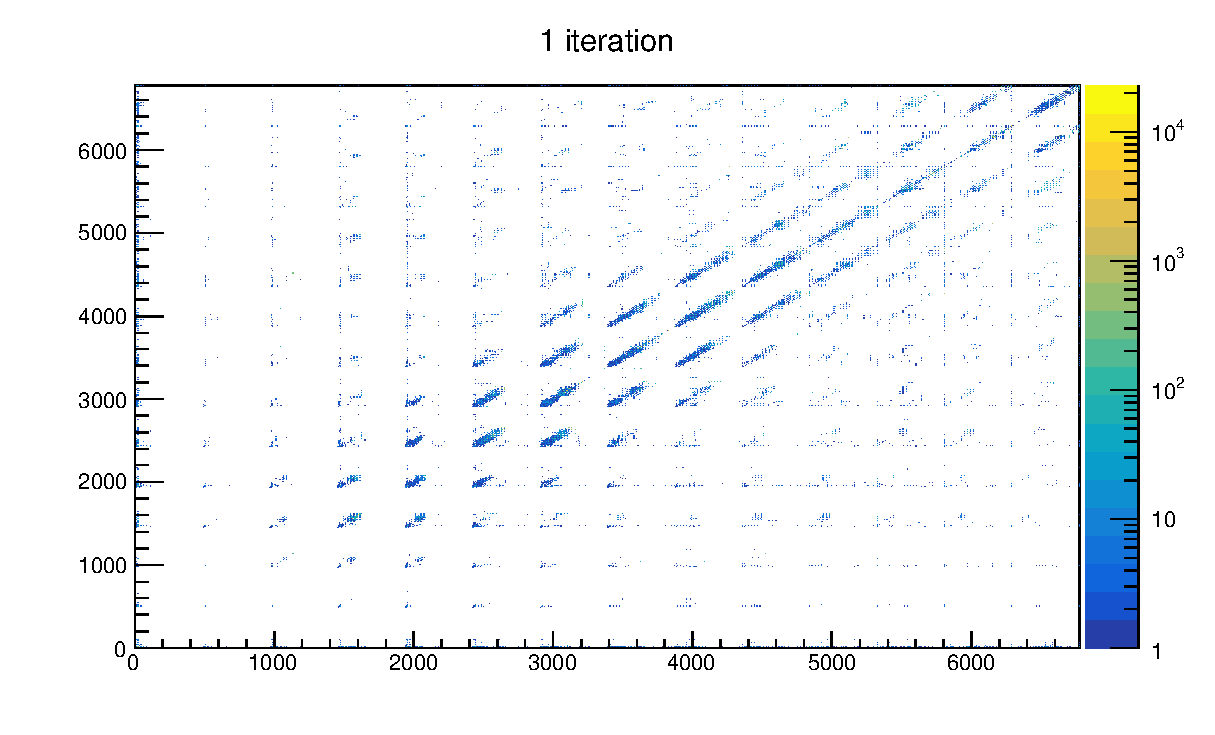
\includegraphics[width=\textwidth]{figures/cov_mat.eps}
  \end{column}
  \begin{column}{.4\textwidth}
    \begin{itemize}
      \item Log scale is used to make the structure more visible.
      \item Obviously this matrix is singular due to rows and columns with elements all zero. Those are unoccupied bins and unavoidable.
    \end{itemize}
  \end{column}
\end{columns}
\end{frame}

\begin{frame}{Metric for Iteration Optimization and\\ Inverting (Nearly) Singular Matrices}
\begin{columns}
  \begin{column}{.5\textwidth}
    \begin{itemize}
      \item For the metric, we use average global correlation coefficient\footnotemark[1].
      \begin{eqnarray*}
        \rho_{avg} &=& \frac{1}{N}\sum^{N}_{j=1}\rho_j \\
        \rho_j &=& \sqrt{1-\frac{1}{[\mathbf{V}]_{jj}[\mathbf{V}^{-1}]_{jj}}}
      \end{eqnarray*}
      , where $j$ runs through all bins and $\mathbf{V}$ the covariance matrix.
    \end{itemize}
  \end{column}
  \begin{column}{.5\textwidth}
    \begin{itemize}
      \item Since $\mathbf{V}$ is singular, I have tried several ways to deal with this.
      \item I tried removing the zero rows and columns. I will talk about this later.
      \item I also tried pseudoinverse (Moore-Penrose inverse). I will not define it, but cite important properties here.
      \begin{enumerate}
        \item For any matrix $\mathbf{A}$, there exists a unique pseudoinverse of it, denoted $\mathbf{A}^+$.
        \item If $\mathbf{A}$ is invertible, $\mathbf{A}^{-1}=\mathbf{A}^+$.
      \end{enumerate}
    \end{itemize}
  \end{column}
\end{columns}
\footnotetext[1]{\href{https://arxiv.org/abs/1611.01927}{Data Unfolding Methods in High Energy Physics}}
\end{frame}

\begin{frame}{Playing with Pseudoinverse}
\begin{columns}
  \begin{column}{.5\textwidth}
    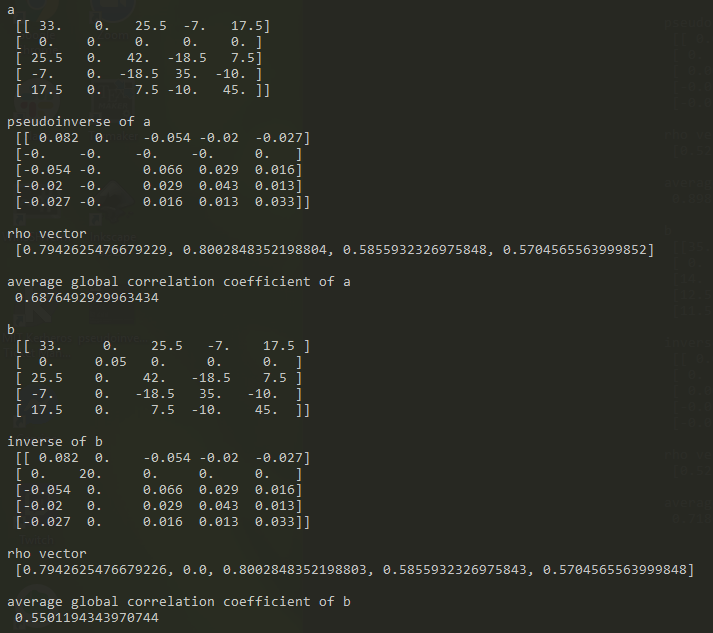
\includegraphics[width=\textwidth]{figures/pseudoinverse_testing.png}
  \end{column}
  \begin{column}{.5\textwidth}
    \scriptsize
    \begin{enumerate}
      \item I generated a random symmetric matrix $\mathbf{A}$, and manually set the second row and column to zero.
      \item The pseudoinverse of $\mathbf{A}$ is calculated.
      \item The $\boldsymbol{\rho}$ vector of $\mathbf{A}$ is calculated.
      \item A second matrix $\mathbf{B}$ is generated by copying $\mathbf{A}$ and setting the $0$ on the diagonal to $0.05$. (Following Matt Judah)
      \item The inverse of $\mathbf{B}$ is calculated.
      \item The $\boldsymbol{\rho}$ vector of $\mathbf{B}$ is calculated.
    \end{enumerate}
    \begin{itemize}
      \item The two results are identical except where they are different to start with.
      \item I did the bench testing because even I made the zero diagonal elements $0.05$ in the real covariance matrices, they were still singular.
%      \item Geometrically, pseudoinverse projects orthogonally to the subspace of the range of the matrix, and invert from there.
    \end{itemize}
  \end{column}
\end{columns}
\end{frame}

\begin{frame}{Nonphysical Values of $\rho_j$'s}
  \begin{itemize}
    \item As the paper and the name (correlation coefficient) suggest, a valid $\rho_j$ should be in the range
    \begin{equation}
      0\le \rho_j=\sqrt{1-\left(\mathbf{V}_{jj}\mathbf{V}^{-1}_{jj}\right)^{-1}} \le 1 \label{rho_range}
    \end{equation}
    \item Eq.~(\ref{rho_range}) is satisfied if and only if
    \begin{equation}
      \mathbf{V}_{jj}\mathbf{V}^{-1}_{jj} \ge 1 \label{valid_v}
    \end{equation}
    \item I went on to use pseudoinverse to calculate $\rho_{avg}$, and found that only a fraction of all $\rho_j$'s satisfy Eq.~(\ref{valid_v}).
    \item I started to suspect that the inverse process involved is numerically unstable.
  \end{itemize}
\end{frame}

\begin{frame}{Condition Number and $\mathbf{V}_{jj}\mathbf{V}^{-1}_{jj}$}
  \begin{itemize}
    \item Consider the linear equation $\mathbf{A}\mathbf{x}=\mathbf{b}$. If small changes in $\mathbf{b}$ imply small changes in the solution $\mathbf{x}$, then $\mathbf{A}$ has a small condition number. Otherwise $\mathbf{A}$ has a big condition number.
    \item Not surprisingly, nearly singular matrices have large condition numbers.
    \item Since I don't know how to prove Eq.~(\ref{valid_v}) mathematically, I did what an experimentalist does: do some experiments.
    \item I generated random positive semidefinite matrices to simulate covariance matrices, and look at their condition numbers and $\mathbf{V}_{jj}\mathbf{V}^{+}_{jj}$'s.
  \end{itemize}
\end{frame}

\begin{frame}[fragile]{Condition Number and $\mathbf{V}_{jj}\mathbf{V}^{-1}_{jj}$ (Cont.)}
  \begin{columns}
    \begin{column}{.5\textwidth}
      \tiny
      \begin{lstlisting}
          well-conditioned example

positive semidefinite matrix V
[[ 80.844 101.687  -7.097   3.693 -37.207]
 [101.687 227.373 -87.639  15.71  -42.425]
 [ -7.097 -87.639 223.402  64.78   61.958]
 [  3.693  15.71   64.78  118.352  24.211]
 [-37.207 -42.425  61.958  24.211  78.489]]

condition number of V
34.26

V_ii*(V^+)_ii
[4.675 4.628 2.953 1.431 2.122]
      \end{lstlisting}
    \end{column}
    \begin{column}{.5\textwidth}
      \tiny
      \begin{lstlisting}
          ill-conditioned example

positive semidefinite matrix V
[[ 53.276 -19.187 -71.864 -33.168 -44.791]
 [-19.187  10.654  23.82    3.057  17.234]
 [-71.864  23.82   98.07   49.632  59.81 ]
 [-33.168   3.057  49.632  41.747  25.265]
 [-44.791  17.234  59.81   25.265  37.982]]

condition number of V
1.582e+17

V_ii*(V^+)_ii
[0.13 0.097 0.204 1.237 0.142]
      \end{lstlisting}
    \end{column}
  \end{columns}
Out of those tens of random positive semidefinite matrices, they showed invariably that,
    \begin{itemize}
      \footnotesize
      \item If the condition number is small (say, $<1000$), $\mathbf{V}_{jj}\mathbf{V}^+_{jj} \ge 1$ is always true for all $j$.
      \item If the condition number is large (i.e., in scientific notation), $\mathbf{V}_{jj}\mathbf{V}^{+}_{jj} \ge 1$ is not satisfied for some or all $j$.
    \end{itemize}
Bottom line: $\mathbf{V}_{jj}\mathbf{V}^{+}_{jj} \ge 1$ is true for all $j$ only if $\mathbf{V}$ is well-conditioned.
\end{frame}

\begin{frame}{Removing Zero Rows and Columns Does Not Help!}
%  \begin{center}
%    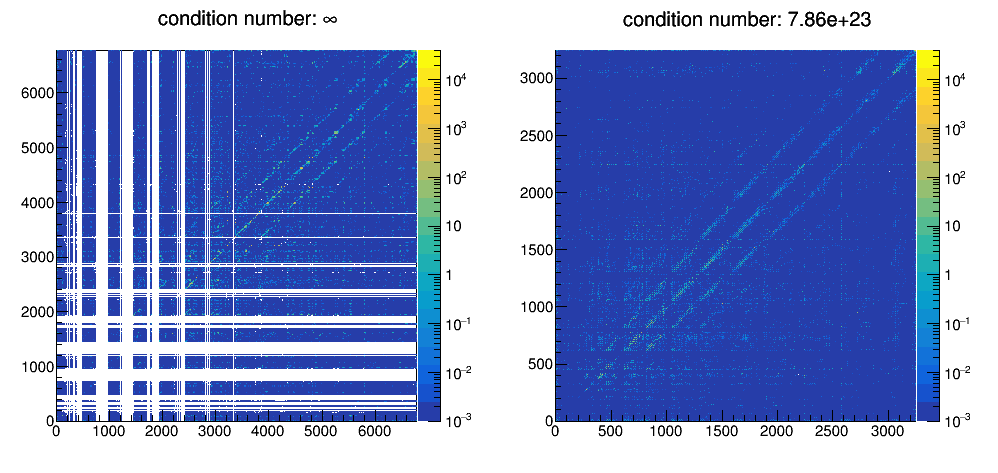
\includegraphics[height=.6\textheight]{figures/iter2tol1e-15.png}
%  \end{center}
  \begin{columns}
    \begin{column}{.68\textwidth}
      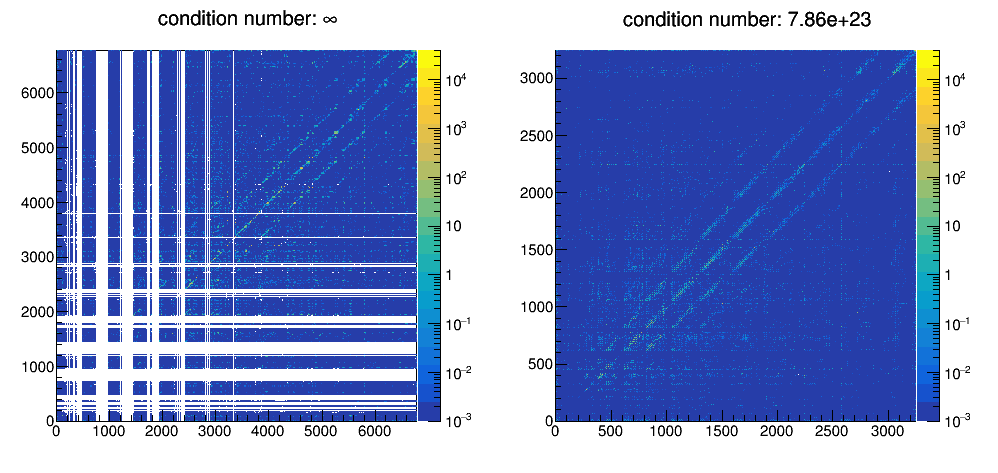
\includegraphics[width=\textwidth]{figures/iter2tol1e-15.png}
    \end{column}
    \begin{column}{.32\textwidth}
      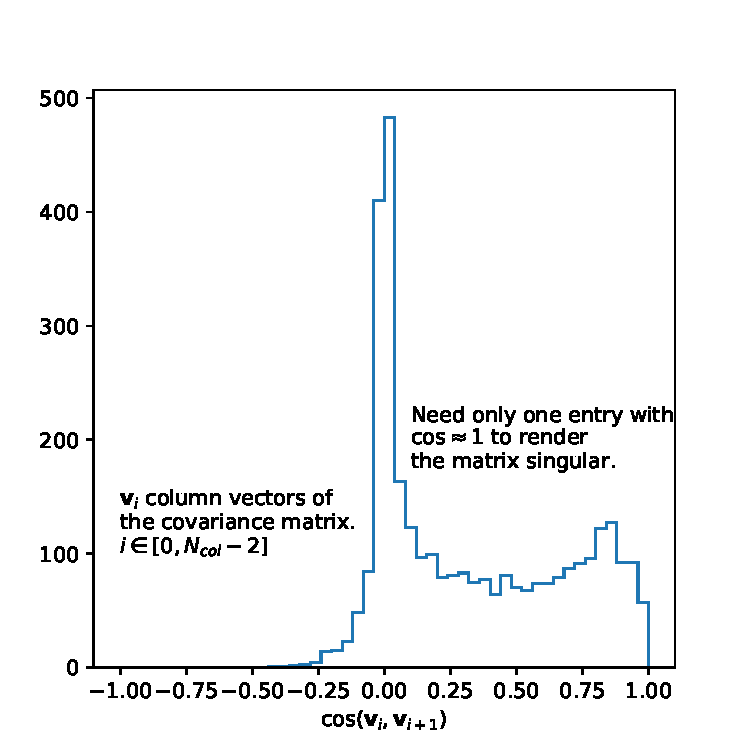
\includegraphics[width=\textwidth]{figures/collinearity.pdf}
    \end{column}
  \end{columns}
  \begin{itemize}
    \scriptsize
    \item Plots are with 2 iterations. Similar situation applies to all iterations.
    \item The reason is a large matrix becomes nearly singular if it contains highly correlated rows or columns. 
    \item The adjacent columns of a covariance matrix are very often highly correlated.
    \item Of course, smaller matrices are always better. Will move to using the zero suppressed matrices.
  \end{itemize}
\end{frame}

\begin{frame}{The Rank and Inverse of a Large Matrix Actually Depend on a Small Tolerance!}
  \begin{itemize}
    \item Intuitively, the number of valid $\rho_j$'s should not exceed the rank of the matrix. Therefore, knowing the rank of the matrix helps understand the problem.
    \item Turns out the rank of a large matrix depends on a small tolerance $\epsilon$. Singular values obtained by SVD (singular value decomposition) that are smaller than $\epsilon$ are set to exact zero to avoid numerical instability. This is called \textcolor{red}{low-rank approximation (or truncated SVD)}, and regarded as a way of regularizing the linear system.
    \item The same tolerance applies to obtaining the pseudoinverse of the matrix since the most common algorithm used to calculated the pseudoinverse is using SVD.
    \item I am going to show you the ranks, the $\rho_{avg}$'s among valid $\rho_j$'s of the covariance matrices as a function of number of iterations and compare results obtained with two different tolerance values.
  \end{itemize}
\end{frame}

\begin{frame}{Different Tolerance Values Result in Different Number of Valid $\rho_j$}
  \begin{columns}
    \begin{column}{.6\textwidth}
      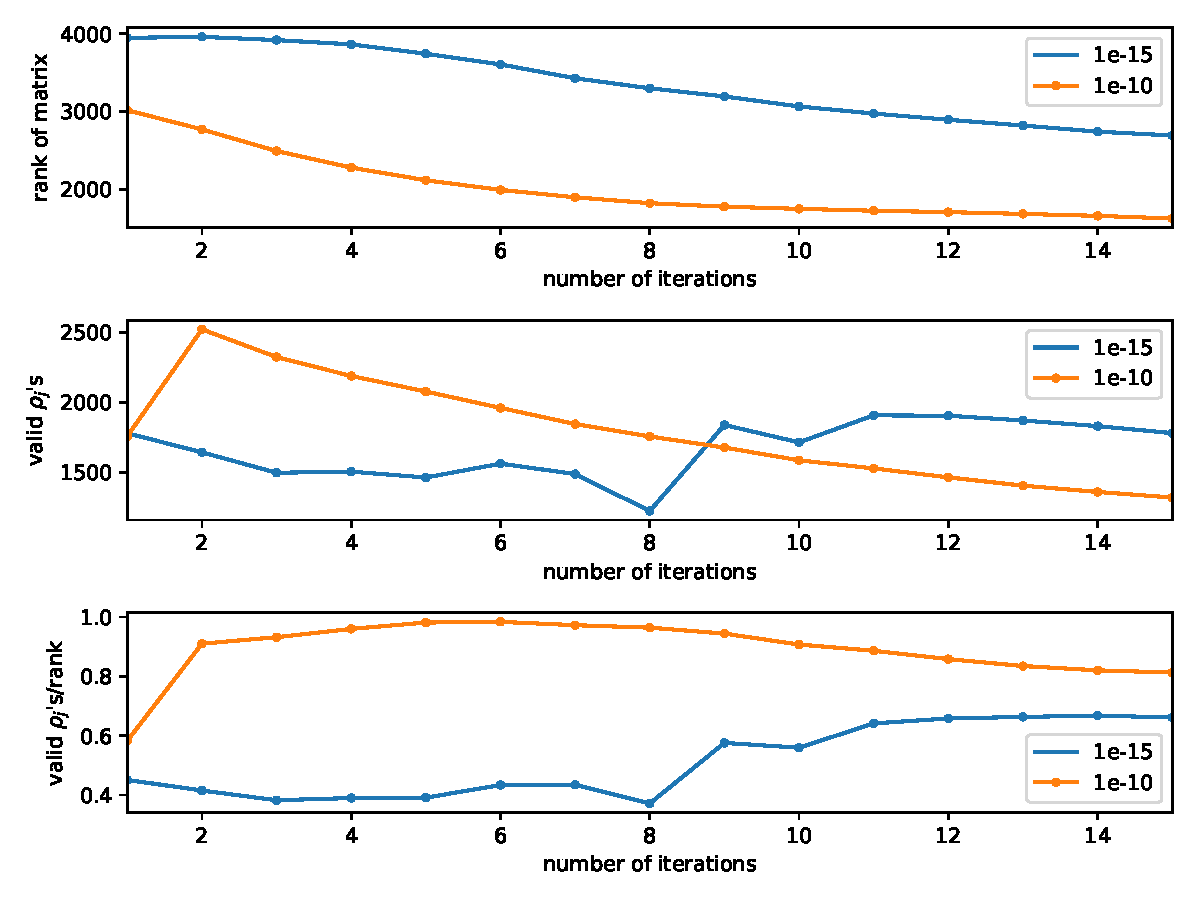
\includegraphics[width=\textwidth]{figures/valid_rank_ratio.pdf}
    \end{column}
    \begin{column}{.4\textwidth}
      \begin{itemize}
        \footnotesize
        \item Different iterations give different covariance matrices.
        \item With $\epsilon=10^{-15}$, some matrices have ranks larger than the size of the zero-suppressed counterparts! This is evidence of numerical instability.
        \item A criterion for how well a matrix is regularized in this study can be \emph{the ratio of the number of valid $\rho_j$'s to the rank.} In this sense, $\epsilon=10^{-10}$ should give a more reliable measure.
      \end{itemize}
    \end{column}
  \end{columns}
\end{frame}

\begin{frame}{$\rho_{avg}$ Results, Work to Do}
  \begin{columns}
    \begin{column}{.55\textwidth}
      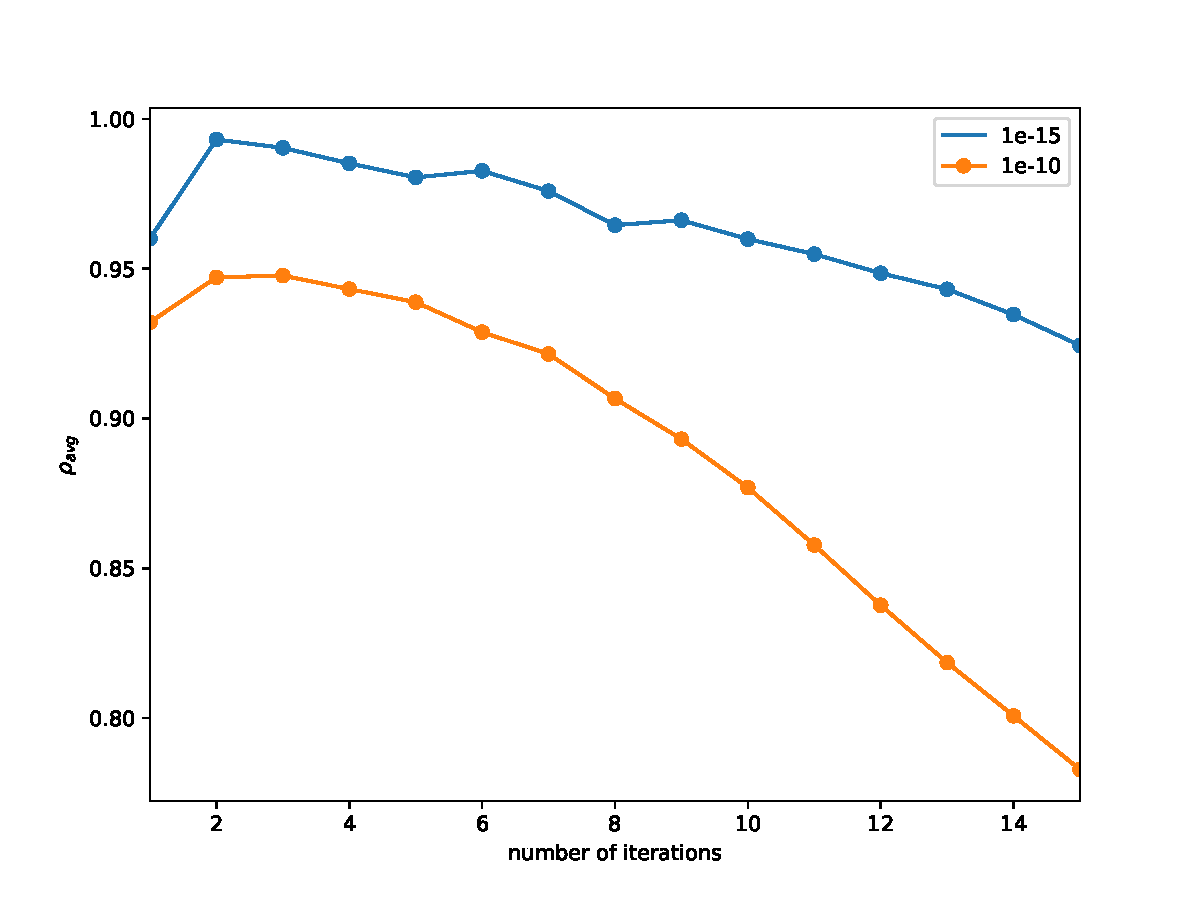
\includegraphics[width=\textwidth]{figures/average_rho.pdf}
    \end{column}
    \begin{column}{.45\textwidth}
      \begin{itemize}
        \small
        \item Although the results depend on tolerance, the \emph{trends} with iterations are the same.
        \item Obviously I need to extend the plots to at least 100. I will sample iterations in $[1,1000]$ and see if a minimum exists.
        \item I have to run the analysis on grid, or implement a much faster covariance matrix calculation algorithm.
        \item If there are any other iteration optimization metrics that are much easier to wield, I am happy to switch over...
      \end{itemize}
    \end{column}
  \end{columns}
\end{frame}

\end{document}